\subsection{Finita volymmetoden}

\newcounter{fvmpauses}
\newcounter{staggeredpauses}

\begin{frame}
\frametitle{Finita volymmetoden}
\begin{columns}[c]

\column{.6\textwidth}
\begin{itemize}[<+(1)->]
\item Finita volymmetoden (Finite Volume Method, FEM)
    \setcounter{fvmpauses}{\thebeamerpauses}
%\item Staggered grid
%    \setcounter{staggeredpauses}{\thebeamerpauses}
\end{itemize}

\column{.45\textwidth}

\begin{figure}
\centering
\uncover<\thefvmpauses->{
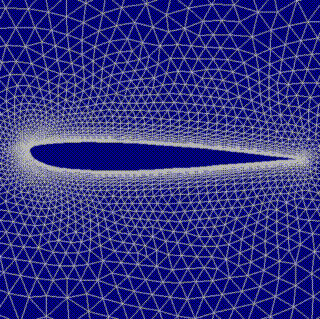
\includegraphics[width=.5\textwidth]{../Presentation/Images/Attribute/Grid/Zhukovskii_profile_by_NASA}
}
\\
\allowbreak 
\end{figure}
%\begin{figure}
%\centering
%\uncover<\thestaggeredpauses->{
%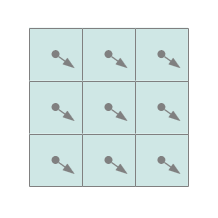
\includegraphics[width=0.35\textwidth]{../Presentation/Images/Attribute/Staggered/Staggered_grid_schema1}
%\quad
%\uncover<\thestaggeredpauses->{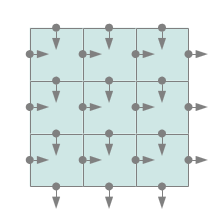
\includegraphics[width=0.35\textwidth]{../Presentation/Images/Attribute/Staggered/Staggered_grid_schema2}}
%}
%\allowbreak 
%\end{figure}

\end{columns}
\end{frame}